% !TeX program = xelatex
% !BIB program = biber
% !TeX spellcheck = es_ES

%------------------
% REQUIREMENTS
%------------------
% The beginning of the document with "\documentclass[aspectratio=169,usenames,dvipsnames]{beamer}" is mandatory since the template has been developed for the 16:9 aspect ratio and requires the "xcolor" and "tikz" packages.

%------------------
% DOCUMENT TYPE
%------------------
\documentclass[aspectratio=169,usenames,dvipsnames,spanish]{beamer}
% Replace "spanish" for "english" or any other language.

%%%%%%%%%%%%%%%%%%%%%%%%%%%%%%%%%%%%%%%%%%%%%%%%%%

%------------------
% DOCUMENT THEME
%------------------
\usetheme{UNAL}



%%%%%%%%%%%%%%%%%%%%%%%%%%%%%%%%%%%%%%%%%%%%%%%%%%


%------------------
% PACKAGES
%------------------
\usepackage{graphics,graphicx} % To insert graphs. They must be in the same folder than the .TEX file.
\usepackage{amsthm, amssymb, amsfonts, latexsym, mathtools,thmtools,bbm} % Enviroments and several math symbols.
\usepackage{ragged2e} % Justifies text.
\usepackage{tikzsymbols} % Emojis.
\usepackage{comment} % To comment huge portions of text.
\usepackage{multicol} % For multiple columns of text or listings.
\usepackage{verbatim} % For code-style text.
\usepackage{listings}
\usepackage{xcolor}

% Define Python syntax highlighting
\lstdefinestyle{pythonstyle}{
    language=Python,
    basicstyle=\ttfamily\footnotesize,
    keywordstyle=\color{blue}\bfseries,
    commentstyle=\color{gray}\itshape,
    stringstyle=\color{red},
    numberstyle=\tiny\color{gray},
    numbers=left,
    numbersep=5pt,
    frame=single,
    breaklines=true,
    breakatwhitespace=true,
    tabsize=4,
    showstringspaces=false,
    captionpos=b
}
% Add any additional packages that are needed here.
%%%%%%%%%%%%%%%%%%%%%%%%%%%%%%%%%%%%%%%%%%%%%%%%%%


%------------------
% INFO
%------------------
\title[Tarea 1]{Tarea 1}
\subtitle{Análisis Numérico, código: 3006886}
\author[Grupo 1]{%
\scriptsize
\setlength{\tabcolsep}{4pt}
\begin{tabular}{p{.31\textwidth}p{.31\textwidth}p{.31\textwidth}}
Haiber Alfredo Alpala Guancha & Maria Paula Ardila Otero & David Delgado Ortiz \\
Juan Pablo Gomez Gomez       & Samuel Mira Alvarez      & Juan Diego Ospina Ocampo \\
Jose Fernando Portilla Rosero& Mariana Valencia Cubillos& Jacobo Zapata Rojas \\
\end{tabular}
}

%\author[Autor]{Autor de la presentación}
\institute{Universidad Nacional de Colombia - Sede Medellín}
\date{\today}
% IMPORTANT: If any of the parameters are too long for the cover or require multiple lines (e.g., extensive title), their arrangement can be modified in the "beamerinnerthemeUNAL.sty" file.
%%%%%%%%%%%%%%%%%%%%%%%%%%%%%%%%%%%%%%%%%%%%%%%%%%
%%%%%%%%%%%%%%%%%%%%%%%%%%%%%%%%%%%%%%%%%%%%%%%%%%
%%%%%%%%%%%%%%%%%%%%%%%%%%%%%%%%%%%%%%%%%%%%%%%%%%


\begin{document}
\justifying % This command justifies all text OUTSIDE of boxes/environments. To also justify text inside boxes/environments, you should use this same command within the box/environment, just right before the text.


%------------------
% COVER
%------------------
\begin{frame}
    \titlepage 
    % The background image, its opacity, and position can be modified in the file "beamerinnerthemeUNAL.sty".
\end{frame}


%------------------
% TABLE OF CONTENTS
%------------------
\begin{frame}{Contenidos}
  \tableofcontents[sections={1}]
\end{frame}

\begin{frame}{Contenidos}
  \tableofcontents[sections={2}]
\end{frame}


%------------------
% Parte 1
%------------------
\section{La cinemática de un brazo robótico}
\framecard{\shadowtext{La cinemática de un brazo}\\\shadowtext{robótico}}
\subsection{Descripción del problema}
\begin{frame}{Descripción del problema}
Considere un brazo robótico planar compuesto por dos eslabones de longitudes \(L_{1}\) y \(L_{2}\), articulados mediante ángulos \(\theta_{1}\) (el que forma el primer eslabón con la base de soporte) y \(\theta_{2}\) (el que forma el segundo eslabón respecto al primero).

\begin{figure}
    \centering
    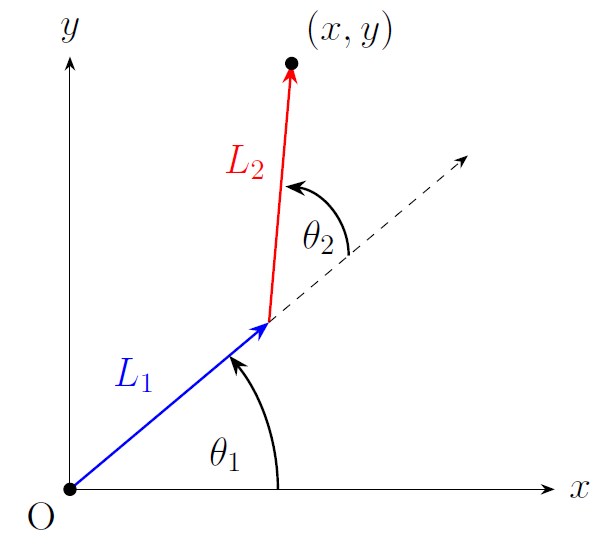
\includegraphics[width=0.35\linewidth]{graphics/grafica_descripcion.png}
\end{figure}  
\end{frame}

\begin{frame}{Descripción del problema}
La posición del extremo del brazo en el plano (en coordenadas cartesianas) está dada por:
\[
x(\theta_{1}, \theta_{2}) = L_{1}\cos(\theta_{1}) + L_{2}\cos(\theta_{1}+\theta_{2})
\]

\[
y(\theta_{1}, \theta_{2}) = L_{1}\sin(\theta_{1}) + L_{2}\sin(\theta_{1}+\theta_{2})
\]

Para alcanzar un punto deseado \((x_{d}, y_{d})\), se plantea el sistema no lineal:
\[
F_{1}(\theta_{1}, \theta_{2}) = x(\theta_{1}, \theta_{2}) - x_{d} = 0
\]
\[
F_{2}(\theta_{1}, \theta_{2}) = y(\theta_{1}, \theta_{2}) - y_{d} = 0
\]
\end{frame}


%------------------
% Punto 1
%------------------
\subsection{Método de Newton para resolver el sistema no lineal}
\begin{frame}{Método de Newton}
    Newton comía manzanas
\end{frame}

%------------------
% Punto 2
%------------------
\subsection{Valores realistas para L1, L2}
\subsection{Tres posiciones destino}
\subsection{Evaluar los resultados del método}
\begin{frame}{Valores realistas para L1, L2}
    
\end{frame}

%%%%%%%%%%%%%%%%%%%%%%%%%%%%%

\begin{frame}{Tres posiciones destino}
    
\end{frame}

%%%%%%%%%%%%%%%%%%%%%%%%%%%%%

\begin{frame}{Resultados del método}
    
\end{frame}

%------------------
% Punto 3
%------------------
\subsection{Sensibilidad de las condiciones iniciales}
\subsection{Casos donde el método converge}
\subsection{Dificultades en la implementación}
\begin{frame}{Sensibilidad condiciones iniciales}
    
\end{frame}

\begin{frame}{Casos donde el método converge}
    
\end{frame}

\begin{frame}{Dificultades en la implementación}
    
\end{frame}


%------------------
% Punto 4
%------------------
\subsection{Visualizar posiciones finales alcanzadas}
\subsection{Visualizar trayectorias intermedias del brazo}
\begin{frame}{Posiciones finales alcanzadas}
    
\end{frame}

\begin{frame}{Trayectorias intermedias del brazo}
    
\end{frame}


%------------------
% Punto 5
%------------------
\subsection{Generalizar el modelo a un brazo con más de 3 eslabones}
\begin{frame}{Generalización más de 3 eslabones}
    
\end{frame}

%------------------
% Parte 2
%------------------

\section{Códigos para resolver sistemas de ecuaciones}
\framecard{\shadowtext{Códigos para resolver}\\\shadowtext{sistemas de ecuaciones}}
%------------------
% Propagación del error
%------------------
\subsection{Propagación del error}
\begin{frame}{Propagación del error}
    
\end{frame}

%------------------
% Bisección
%------------------
\subsection{Bisección}
\begin{frame}{Método de bisección}
    
\end{frame}

%------------------
% Punto fijo
%------------------
\subsection{Punto fijo}
\begin{frame}{Método del punto fijo}
    
\end{frame}

%------------------
% Newton
%------------------
\subsection{Newton}
\begin{frame}{Método de Newton}
    
\end{frame}

%------------------
% Newton modificado
%------------------
\subsection{Newton modificado}
\begin{frame}{Método de Newton modificado}
    
\end{frame}

%------------------
% Secante
%------------------
\subsection{Secante}
\begin{frame}[fragile]{Método de la secante}
\lstset{
    language=Python,
    basicstyle=\ttfamily\tiny,
    keywordstyle=\color{blue}\bfseries,
    commentstyle=\color{gray}\itshape,
    stringstyle=\color{red},
    numberstyle=\tiny\color{gray},
    numbers=left,
    numbersep=3pt,
    frame=single,
    breaklines=true,
    breakatwhitespace=true,
    tabsize=2,
    showstringspaces=false
}

\begin{lstlisting}
from typing import Callable, TypedDict
import numpy as np

class SecantMethod(TypedDict):
    solution: int
    message: str

def secante(f: Callable[[float], float], x0: float, x1: float,
           delta: float = 1e-5, max_iterations: int = 1000) -> SecantMethod:
    if x1 == x0:
        raise ValueError("Initial guess x0 and x1 must be different")
    
    for i in range(max_iterations):
        df_numeric = (f(x1) - f(x0)) / (x1 - x0)
        x = x1 - f(x1) / df_numeric
        
        if np.abs(f(x)) < delta:
            return {"solution": float(x), 
                   "message": f"Converged after {i+1} iterations"}
        
        x0, x1 = x1, x
    
    return {"solution": float(x), 
           "message": "Max iterations exceeded"}
\end{lstlisting}
\end{frame}


%------------------
% Agradecimiento
%------------------
\framepic[0.6]{graphics/BibliotecaMedellin.jpg}{
    \framefill
    \textcolor{black}{%
    \scshape
    \shadowtext{Muchas gracias}\\
    \shadowtext{por su atención}
    }%
    \vskip 1cm
}







% Comentar desde este punto hasta "\end{frame}" para no mostrar referencias. Esto se debe hacer sólo si NUNCA se usó el comando \cite en las diapositivas.
%\section{Referencias}
%\begin{frame}[allowframebreaks]
%\frametitle{Referencias}
%\bibliographystyle{amsalpha} %Estilo bibliografía.
%{\scriptsize \justifying
%\bibliography{References}}
%\end{frame}

\end{document}
%%%%%%%%%%%%%%%%%%%%%%%%%%%%%%%%%%%%%%%%%%%%%%%%%%
%%%%%%%%%%%%%%%%%%%%%%%%%%%%%%%%%%%%%%%%%%%%%%%%%%
%%%%%%%%%%%%%%%%%%%%%%%%%%%%%%%%%%%%%%%%%%%%%%%%%%